
\documentclass{amsart}
\usepackage{graphicx}
\usepackage{amsmath}
\usepackage{bbold}
\usepackage{lipsum}
\usepackage{xpatch}
\xpatchcmd{\paragraph}{\normalfont}{{\normalfont\bfseries}}{}{}

\newtheorem{theorem}{Theorem}[section]
\newtheorem{lemma}[theorem]{Lemma}

\theoremstyle{definition}
\newtheorem{definition}[theorem]{Definition}
\newtheorem{example}[theorem]{Example}
\newtheorem{xca}[theorem]{Exercise}
\newtheorem*{prop*}{Proposition}
\theoremstyle{remark}
\newtheorem{remark}[theorem]{Remark}

\numberwithin{equation}{section}

%    Absolute value notation

\newcommand{\abs}[1]{\lvert#1\rvert}
\newcommand\norm[1]{\left\lVert#1\right\rVert}

%    Blank box placeholder for figures (to avoid requiring any
%    particular graphics capabilities for printing this document).
\newcommand{\blankbox}[2]{%
  \parbox{\columnwidth}{\centering
%    Set fboxsep to 0 so that the actual size of the box will match the
%    given measurements more closely.
    \setlength{\fboxsep}{0pt}%
    \fbox{\raisebox{0pt}[#2]{\hspace{#1}}}%
  }%
}

\DeclareMathOperator*{\argmin}{argmin} 



\begin{document}

\title{High-dimensional Estimation With Geometric Constrains: Report}

%    Information for first author
\author{Parnian Kassraie}
%    Address of record for the research reported here
\address{Compressed Sensing, Sharif University of Technology, Spring 2018}

\email{kasraei\_parnian@ee.sharif.edu}

\maketitle

\specialsection*{\textbf{Introduction}}
Briefly explained, This paper introduces a simple and general estimator of a $x$, where $x$ can be any vector or signal with any geometric constraints, coming from a model $f$, where $f$ can be a nonlinear semi-parametric single-index model. The problem can include additive or non-linear noise.\\
Later an upper error bound is proven for their estimator, with a nice geometric interpretation for the error and minimum number of samples need for controlling that error up to a constant value.\\
Min-max optimality of the estimator for linear and nonlinear models is discussed under certain geometric condition and for specific $f$s, again, with a neat geometric analogy.
\par This report with include a concise summery of the paper as well as a detailed section on my contribution that was presented in class.\\
\begin{quotation}
The Reader can easily skip Paper Summery (section 1) and start reading from the Matrix Completion (section 2) which is my additional contribution to the paper.
\end{quotation}
\section{\textbf{Paper Summery}}
\subsection{The Model \& It's Upper Error Bound}
The following model is used throughout the paper:
\[
y_i = f(\langle a_i,x \rangle +\epsilon),\quad 1\leq i \leq m
\]
Where $f:\mathbb{R}\rightarrow \mathbb{R}$ is an unknown function, $x\in \mathbb{R}^n$ is the fixed unknown signal and $a_i \sim \mathcal{N}(0,I_n) $ are i.i.d random variables, the observation or sensing vectors. Therefore,
\begin{quote}
each observation $y_i$ may depend on $a_i$ only through $\langle a_i,x\rangle$
\end{quote}
In our problems, often we have a prior knowledge of $x$. This information is modeled by saying $x \in K$. Further on, we will assume that $K$ is a Star-shaped ($\forall \,\, 0\leq \lambda \leq 1: \lambda K \subseteq K$) subset of $\mathbb{R}^n$.

Now let's see how we can estimate $x$.
\subsubsection{\textbf{Linear Estimator}} 
The simplest approach is to ignore $K$, which is common in ML estimations. The linear estimator is then defined as:
\[
\hat{x}_{lin} := \frac{1}{m} \sum_{i=1}^m y_i a_i
\]
It can be seen that it's an unbiased estimator of normalized $x$. For the error bound we have the following theorem:
\begin{theorem}
\[
\mathbb{E} \hat{x}_{lin} = \mu \bar{x},\quad \sqrt{\mathbb{E}\norm{\hat{x}_{lin}-\mu\bar{x}}_2^2} = \frac{1}{\sqrt{m}}[\sigma+\eta\sqrt{n}]
\]
Where
\[
\bar{x} = \frac{x}{\norm{x}_2},\quad \mu = \mathbb{E}y_1<a_1,\bar{x}>,\quad \sigma^2= Var(y_1<a_1,\bar{x}),\quad \eta^2 = \mathbb{E} y_1^2
\]
\end{theorem}

Proof can be found in the paper, section 8.2.\\
\par Now let's explore the estimator introduced in the paper, but before, we have to get familiar with concept of mean width.

\subsubsection{\textbf{Mean Width}}  The width of K in the direction of a given unit vector $\eta\in S^{n-1}$ is defined as the width of the smallest slab between two parallel hyperplanes with normals $\eta$ that contains $K$; Figure 1.We can express the width in the direction of η as 
\[
\sup_{u,v \in K} \langle \eta, u-v \rangle = \sup_{z \in K-k} \langle \eta, z \rangle
\]
where $K −K = \{u − v : u, v \in K\}$ is the Minkowski sum of $K$ and $−K$. Averaging over $\eta$ uniformly distributed on the sphere $S^{n−1}$, we can define the spherical mean width of $K$:
\[
\tilde{w}(K) :=\mathbb{E} \sup_{z\in K−K} \langle \eta , z\rangle \]

\begin{definition}[Gaussian Mean Width]
 The Gaussian mean width of a bounded subset $K$ of $\mathbb{R}^n$ is defined as
\[w(K) :=\mathbb{E} \sup_{u\in K − K} \langle g, u \rangle \]
where $ g \sim \mathcal{N}(0, I_n)$ is a standard Gaussian random vector in $\mathbb{R}^n$. We will refer to Gaussian mean width as simply the mean width.
\end{definition}

\begin{figure}[tb]
%\blankbox{.6\columnwidth}{5pc}
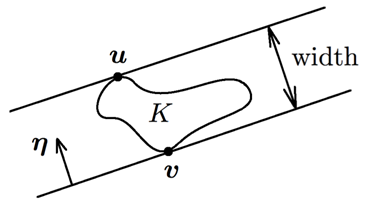
\includegraphics{meanwidth.png}
\caption{Mean Width Illustration}
\label{firstfig}
\end{figure}

Local Mean Width is often used in this paper's theorems, so we'll quickly define it as well:
\[
w_t(K) = \mathbb{E}_g \, \sup_{x,y\in K} \langle g,x-y\rangle ,\quad \norm{x-y}_2\leq t
\]
Some examples of famous mean widths:
\begin{itemize}
\item $B_2^n$:
\[
w(K) = \mathbb{E}_g 2 \norm{g}_2 = 2\sqrt{n}
\]
\item A subset of $B_2^n$ with linear algebraic dimension d:
\[
w(K) = 2 \sqrt{d}
\]
\item A finite subset of $B_2^n$:
\[w(K) = C\sqrt{\vert K \vert}
\]
\item $\Sigma_k \cap S^{n-1}$:
\[
w(K) \leq C \sqrt{s \log 2n/s}
\]
\end{itemize}

\subsubsection{\textbf{Projected Estimator \& Error Bound}}

The straight forward step took in the paper towards improving the linear estimator, is simply projecting it onto the feasible set $K$.
\[
\hat{x} = P_K(\hat{x}_{lin}) = \argmin_{z \in K} \norm{\hat{x}_{lin}-z}_2
\]
The main result of the paper is the upper error bound for projected estimator:
\begin{theorem}(Main Result)
For every $t>0$:
\[
\mathbb{E}\norm{\hat{x}-\mu\bar{x}}\leq t+ \frac{2}{\sqrt{m}}\bigg[ \sigma + \eta \frac{w_t(K)}{t}\bigg]
\]
Optimizing equation above on $t$:
\[
\mathbb{E}\norm{\hat{x}-\mu\bar{x}} \leq \frac{2\sigma}{\sqrt{m}} + 2\sqrt{2}\bigg[\eta \frac{w(K)}{\sqrt{m}}\bigg]^{1/2}
\]
Where $\mu,\eta,\sigma$ are defined similar to the linear case.
\end{theorem}

The theorem shows that in order to have a constant error rate, the sample size ($m$) should be as large as mean width of $K$ squared. Which is a nice reduction for the inherently sparse feasible sets.\\
In the following we will see a couple of examples for better understanding of this abstract model.
\paragraph{Examples of common in practice feasible sets:}
\begin{itemize}
\item Sparse Vectors
\[
K = \Sigma_s
\]
\[
w(K)\leq C \sqrt{s\log \frac{2n}{s}}
\]
\[ m = O(s\log \frac{2n}{s})\]
\item Approximately Sparse Vectors
\[ K = \{v \in \mathbb{R}^n: \norm{v}_1\leq s \}\]
\[ w(K) \leq 4 \sqrt{2 s \log n}\]
\[ m = O(s \log n)\]
\end{itemize}
\paragraph{Examples of common in practice $f-$Models:}
\begin{itemize}
\item Noisy Linear Model
\[
y_i = \langle a_i,x \rangle+\epsilon_i,\quad \epsilon_i \sim \mathcal{N}(0,\nu^2)
\]
The error bound would become:
\[
\mathbb{E}\norm{\hat{x}-\mu\bar{x}} \leq t + \frac{\norm{x}_2+v}{\sqrt{m}}\bigg[1+\frac{w_t(K)}{t}\bigg]
\]
The power of this could be seen when the noise energy is comparable to the signal ($\norm{x}_2+v$ term), the error rate will not increase dramatically and the estimator, to some extent, would still be valid.
\item Non-linear Model
\[
y_i = f(\langle a_i,x \rangle)
\]
If we calculate $\eta,\sigma$ for this setting, we would have:
\[
\sigma^2 = Var\big[f(g\norm{x}_2)g\big],\quad \eta^2 = \mathbb{E}f(g\norm{x}_2)^2
\]
Where $g\sim\mathcal{N}(0,1)$. Recalling the main theorem:
\[
\mathbb{E}\norm{\hat{x}-\mu\bar{x}}\leq t+ \frac{2}{\sqrt{m}}\bigg[ \sigma + \eta \frac{w_t(K)}{t}\bigg]
\]
For heavy-tail nonlinear $f$, we will thus have a looser error bound.

\end{itemize}
\subsection{Model Optimality}
Projected estimator error bound is compared with a general lower bound for \textbf{any estimator} that is only a function of $y_i,a_i$. By comparing these bounds, to sufficient number of samples in order to have a minimax optimal error is calculated. Meaning, having this many samples, there exists no other estimator that could perform orders of magnitude better than the projected estimator, because the projected estimator's upper error bound is controlled by the general lower bound up to a constant factor.

\paragraph{Packing Number} In order to understand the lower error bound we need to introduce the following notation.
\begin{definition}(Packing Number)
Packing number of $K$ with balls of radius $t$:
\[
\mathbb{P}_K = \sup_{\chi} \vert \chi \vert
\]
Where,
\[
\chi \subset K: \,\, \norm{v-w}_2 \geq t,\quad \forall v,w\in \chi.
\]
\end{definition}
Figure 2 can give a geometric understanding of the concept.
\begin{figure}[tb]
%\blankbox{.6\columnwidth}{5pc}
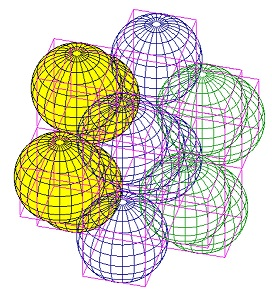
\includegraphics{packing.jpg}
\caption{Pakcing Number Illustration}
\label{firstfig}
\end{figure}

Similar to mean width, Local Packing Number is defined as:
\[
\mathbb{P}_t = \mathbb{P}_{K\cap tB_2^n}
\]
with balls of radius $t/10$. A useful parameter is local packing number to local mean width ratio which will be used later:
\[
\alpha = \alpha(K) = \sup_t \frac{w_t(K)}{t\sqrt{\log P_t}}
\]
\subsubsection{\textbf{Linear Model Optimality}}

\begin{theorem} (Linear Model Lower Error Bound)
For Any $\hat{x}$ which depends only on $y_i,a_i$
\[
\delta_* := \inf_{t>0} \{ t + \frac{\nu}{\sqrt{m}} [ 1+ \sqrt{\log P_t} ] \}
\]
\[
\sup_{x\in K} \mathbb{E}\norm{\hat{x}-x}_2 \geq c \min\big(\delta_*, diam(K)\big)
\]
\end{theorem} 
We 
The main result theorem can be re-written in a way that is similar to the lower bound theorem above:
\[
\mathbb{E}\norm{\hat{x}_{proj}-x}_2 \leq C \inf_t \lbrace t + \frac{\nu + \norm{x}_2}{\sqrt{m}}\big[ 1+ \frac{w_t(K)}{t}\big] \rbrace = C \delta^*
\]
\[
\sup_{x\in K} \norm{\hat{x}_{proj}-x}_2 \leq c \min\big(\delta^*, diam(K)\big)
\]
It can be easily seen that projected estimator for linear models is optimal if:
\[\delta_* \geq \delta^*/\alpha\]
Where $\alpha$ is the radio defined in the previous section. Therefore, for all feasible sets that $\alpha(K)$ is controlled by a constant value the model is optimal, thus a great choice among all estimators. I must mention that such feasible sets aren't hard to find, sparse vectors, low-rank matrices and approximately sparse vectors are some familiar examples.\\
In addition Near-Optimality holds for non-linear models in special cases of $f,K$ which is skipped here since it wasn't included in the presentation.

\section{\textbf{An Application Extending the Paper: Matrix Completion}}

\subsection{The Matrix Completion Problem}

As a practical addition to the paper, I decided to apply the Projected Estimator on Low-Rank Matrix Completion Problem. 

Low-rank Matrix $X \in \mathbb{R}^{d_1 \times d_2}, \, rank(X)\leq r$ is partially observed. The index of observed cells are members of $\Omega \subset \{1,\cdots,d_1\}\times\{1,\cdots,d_2\} $.\\
We define $\Delta$ as the observation mask matrix,
\[
(\Delta)_{ij} = \mathbb{1}_{(i,j)\in \Omega}
\]
Thus, The observed matrix can be formulated as:
\[
X_{obs} = X \circ \Delta
\]
Where $\circ$ is the Hadamard (Entry-wise) product of the two matrices.


Now let's see the estimator this paper suggests for estimating $X$.
\subsection{Plan's Suggested Solution} The linear unbiased estimator for $X$ is $\hat{X}_{lin}=X_{obs}$. However, we know that $X$ is low-rank. Thus, $X\in K$ where
\[
K = \{ M\in \mathbb{R}^{d_1 \times d_2}: \, rank(M)\leq r\}
\]
Therefore, Plan's Estimator would be:
\[
\hat{X} = P_k(\hat{X}_{lin})
\]
Basically, we should simply project the observed matrix onto the set of low-rank matrices. The estimation error, $\norm{X-\hat{X}}_2$ is bounded the squared mean width of this set, which is $W^2(K)\leq 2r(d_1+d_2)$.

\paragraph{Issues} As you might have noticed, projecting $X_{obs}$ onto $K$ would change the value of observed cells. In many of the applications, e.g. Image Reconstruction, preserving the observed information is a necessity. Thus, Plan's Estimator wouldn't be a wise option here.\\
Consistency is an important feature of an estimator, which has received no attention throughout the paper. As explained above, the suggested paper is an unbiased estimator that will not converge to $X$ in the asymptotic setting of,
\[d_1,d_2,r\rightarrow\infty,\,\, \frac{r}{d_1},\frac{r}{d_2}\in [0,1]\]
as long as $r < \min(d_1,d_2)$. This really is an unpleasant property!

\subsection{The Alternative Solution} A simple solution to the issue above, would be projecting $\hat{X}$ onto W,
\[
W = \{M\in \mathbb{R}^{d_1 \times d_2}, \, M_\Omega = X_\Omega \}
\]
Which is an Affine space containing the matrices with correct cells at the observed indices. Projection onto W however, might push the estimator out of $K$. We should look for matrices inside $K\cap W$. 
\paragraph{Main Idea} We keep projecting $\hat{X}_{lin}$ onto $K,W$ repeatedly, for as many times as desired, finishing with a projection to $W$. The method is illustrated in Figure 3. In the following I will show how this method improves the original estimator in theory and in practice.

\begin{figure}[tb]
%\blankbox{.6\columnwidth}{5pc}
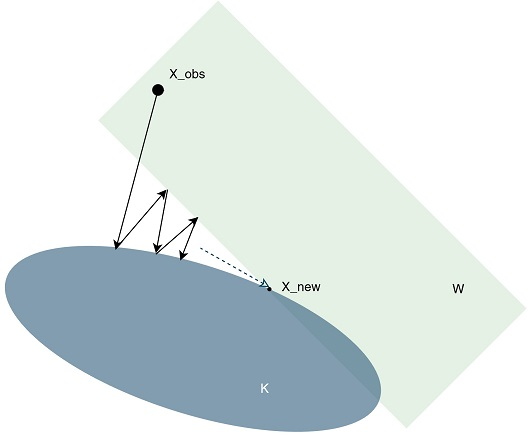
\includegraphics{Proj.jpg}
\caption{Alternative Method}
\label{firstfig}
\end{figure}

\subsubsection{\textbf{Solving the Consistency Issue}} Assuming that $K\cap W\neq \O$, since the real $X\in K\cap W$, the alternative method will tend to find it. In case of $K\cap W=\O$ this method will try to find $\hat{X}_{new}$, where
\[
\hat{X}_{new} = \argmin_{M\in W} \{\min_{N\in K} \norm{M-N} \}
\]
The following proposition will prove consistency of this estimator in the cases where both $W,K$ are convex set. Notice that in our example $K$ is not convex.

\begin{theorem}
For compact convex spaces A, B,  where $A \cap B \neq \O $, By starting from a given point $x$, and periodically projecting it onto A and B, the sequence of resulting points $\{x_i\}$ will converge to a point inside $A \cap B $, where $\{x_i\}$ can be formulated as:
\[
x_0:x,\,\, x_1:P_A(x_0),\,\,x_2:P_B(x_1),\,\,x_3:P_A(x_2),\cdots
\]

\end{theorem}
\begin{lemma}
Given $x,y\in \mathbb{R}^n$ and the compact convex set $C$ we have:
\[
\norm{P_C(x)-P_C(y)}\leq \norm{x-y}
\]
Where $\norm{.}$ is the $l_2$ norm.

\end{lemma}

The proof is skipped since it could be easily derived or found online.

\begin{definition}
Distance of a point from a set is defined as:
\[
d(x,C) = \min_{y \in C} \norm{x-y}
\]
\end{definition}
\begin{lemma}
For $A,B,\{x_i\}$ defined in Theorem 2.2, the sequence $\alpha_n= d(x_n, A\cap B)$ is decreasing.
\end{lemma}
\begin{proof}
Without a loss of generality, assume that $x_{n+1}=P_A(x_n)$. We define $y=P_{A\cap B}(x_n)$, But $y\in A$ hence $P_A(y)=y$. From Lemma 2.3:
\[
d(x_{n+1},A\cap B)\leq \norm{x_{n+1}-y}\leq \norm{x_n-y}=d(x_n,A\cap B) 
\]
\[
d(x_{n+1},A\cap B)\leq d(x_n,A\cap B)
\]
\end{proof}

The only step left to prove Theorem 2.2 is to show convergence of $d(x_n,A\cap B)$ to zero.

\begin{proof}[Proof Theorem 2.2]

\[
\exists \, \epsilon \,\, \text{s.t.} \,\, \forall n\in \mathbb{N}\,\,d(x_n,A\cap B)>\epsilon
\]
Given convex compact set $C$ and point $x$ outside $C$: 
\[
\begin{split}
& P(x) = \argmin_{y\in C} \norm{y-x}^2\\ \Rightarrow & \, \angle yP(x)x\geq\pi/2\\
\Rightarrow & \,\norm{x-y}^2\geq \norm{x-P(x)}^2+\norm{y-P(x)}^2
\end{split}
\]
\begin{figure}[tb]
%\blankbox{.6\columnwidth}{5pc}
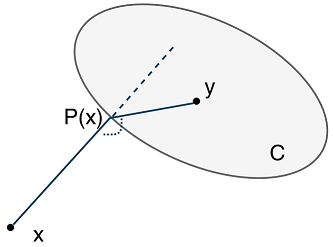
\includegraphics{proof1.png}
\caption{Theorem 2.2 Proof}
\label{firstfig}
\end{figure}
The equations above are illustrated in Figure 4.\\
Therefore if the contradictory assumption holds, we propose that for a sample point $x^*$ in $A\cap B$ the sequence $\norm{x_n-x^*}$ is decreased by $\delta^2$ with every projection. Where $\delta$ is the shortest distance between $A/(A\cap B)_\epsilon$ and $B$ or reverse.\\
On each step $x_i$ is either inside $A/(A\cap B)_\epsilon$ or $B/(A\cap B)_\epsilon$ and is being projected on $B$ or $A$ respectively. Assume the first case, since $A/(A\cap B)_\epsilon \cap B = \O$ then $d(x_i,B)\geq \delta$ thus, $d(x_i,A\cap B)$ is reduced by $\delta^2$. (Check out Figure 5.) The opposite hypothesis is not true and the proposition is proven:
\[
d(x_n,A\cap B) \xrightarrow{n\rightarrow \infty} 0
\]

\begin{figure}[tb]
%\blankbox{.6\columnwidth}{5pc}
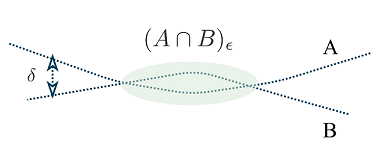
\includegraphics{proof2.png}
\caption{Theorem 2.2 Proof}
\label{firstfig}
\end{figure}

The last step is to prove the sequence $\{x_i\}$ converges to a point inside $A\cap B$, which is done by showing it's Cauchy sequence. \\
For $\epsilon>0,\, \exists x_n,\,x^*\in A\cap B$ that $\norm{x_n-x^*}\leq \epsilon$, thus $\forall m\geq n:\, \norm{x_m-x^*}<\epsilon$. Therefore, all the following members of the sequence are inside a ball centered at $x_n$ with radius $\epsilon$ and the sequence is Cauchy. \\

Convergence of $\{x_i\}$ to $A \cap B $ is thus proven.
\end{proof}
\subsubsection{\textbf{Implementation}} It's a well-known fact that images are low-rank matrices, thus the estimator is implemented in MATLAB as a method for partially observed image reconstruction.\\
Projection onto the space of low-rank matrices is done by calculating SVD and keeping the $r-$largest eigenvalues i.e.  $r-$largest cells on $\Sigma$'s diagonal where $X=U \Sigma V^T$. A few points about the simulations:\\
\begin{itemize}
\item The original image's dimensions are $854\times 1280$.
\item For $r \in \{3,10,50,100\}$, each time $m = O(r(d_1+d2))$ pixels are observed.
\item The indices ($\Omega$) are independent uniform random variables.
\item The final reported SNRs are calculated by averaging on the SNRs of 10 different instances of $\Omega$.
\item The algorithm has 20 projection steps between $K,W$.
\end{itemize}

\paragraph{Results} Original image is shown in Figure 6. Figure 7 shows the result of implementing Plan's estimator and Figure 8 shows the result of implementing the alternative estimator. The codes can be found in \textit{ImageRecovery.m}.

\begin{figure}[tb]
%\blankbox{.6\columnwidth}{5pc}
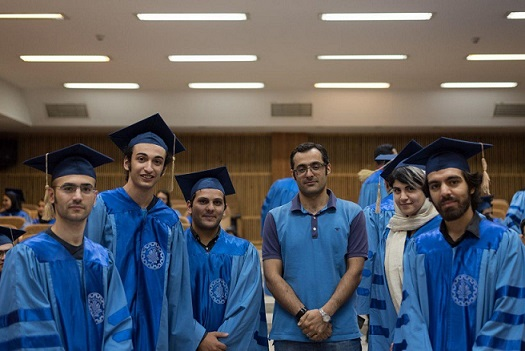
\includegraphics{orig.jpg}
\caption{Original image selected for partial observations}
\label{firstfig}
\end{figure}

\begin{figure}[tb]
%\blankbox{.6\columnwidth}{5pc}
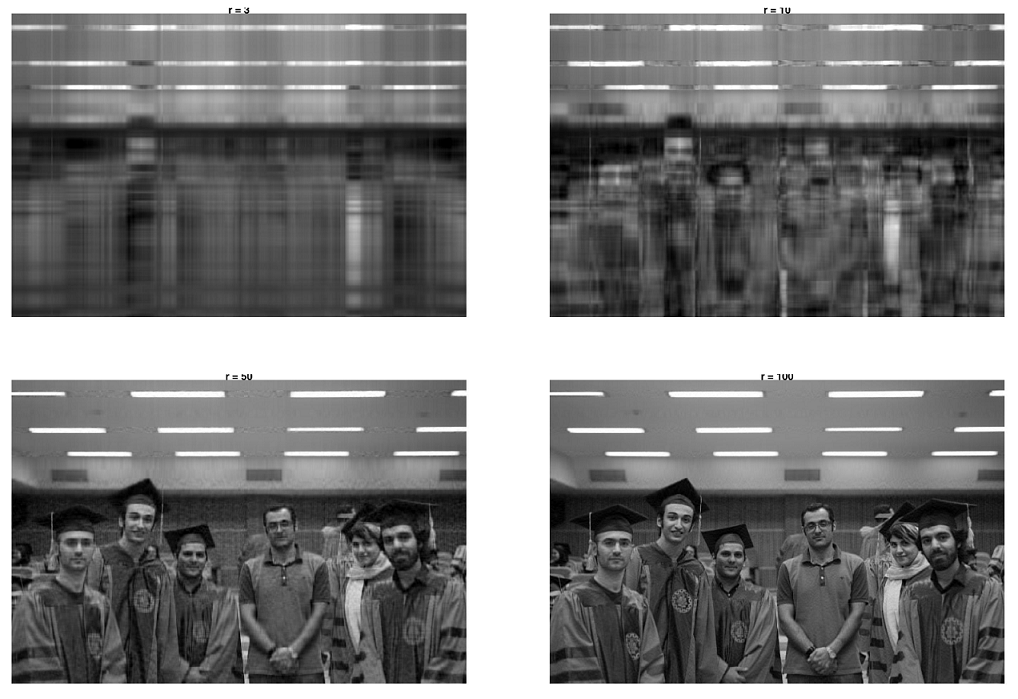
\includegraphics{Plans.png}
\caption{Projected Estimator for Low-rank Matrix Recovery}
\label{firstfig}
\end{figure}

\begin{figure}[tb]
%\blankbox{.6\columnwidth}{5pc}
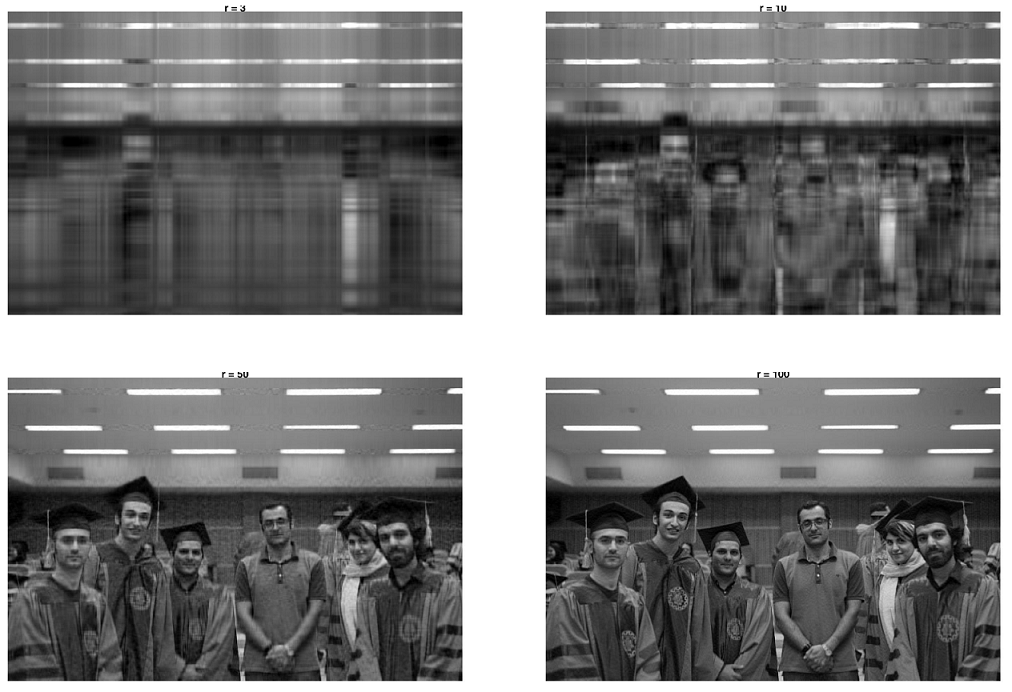
\includegraphics{Parnians.png}
\caption{Projected Estimator for Low-rank Matrix Recovery}
\label{firstfig}
\end{figure}

I have chosen SNR as an indicator for quality of estimation. Table 1. shows how the alternative method improves Plan's estimator for larger assumed image matrix ranks.

\begin{table}[ht]
\caption{SNR Comparison for different assumed ranks}\label{eqtable}
\renewcommand\arraystretch{1.5}
\noindent\[
\begin{array}{|c|c|c|}
\hline
\text{Rank}&\text{Plan's}&\text{Ours}\\
\hline
{3}&-40.5565& -41.6303\\
{10}&1.0223&1.1253\\
{50}&0.9369&0.9292\\
{100}&2.9225 &2.9389\\ 

\hline
\end{array}
\]
\end{table}

A pivotal idea in the paper, is bounding the estimation error with mean width of $K$ and thus, coming up with minimum number of observations needed for controlling the error up to a constant value. In Table 2 I have assumed $r=50$ and then compared the average SNR for Plan's method with different orders of observation. As it can be seen, the suggested order(around 100 thousand samples) significantly improves $O(1)$ and is almost as good as observing all the cell values (about 1 million samples).
\begin{table}[ht]
\caption{SNR Comparison for different number of observations, using Plan's estimator}\label{eqtable}
\renewcommand\arraystretch{1.5}
\noindent\[
\begin{array}{|c|c|c|}
\hline
{\text{order of } m}&{\text{Avg. SNR}}\\
\hline
{\text{Const. Rate}}&  -50.2226\\
{r(d_1+d_2)}&0.9369\\
{d_1d_2}&0.9409 \\

\hline
\end{array}
\]
\end{table}


\paragraph{Further Improvements} The astute reader might have noticed that the proven theory was only on convex compact sets, while we are dealing with non-convex set of low-rank matrices in our problem formulation and implementations. A nice way to remove this problem would be using a convex relaxation of $K$:
\[
\tilde{K}=\{ M \in \mathbb{R}^{d_1 \times d_2} : \norm{M}_* \leq r \}
\]


Where $\norm{.}_*$ is the matrix nuclear norm. (It is only defined for positive definite matrices, but well.) This method was simultaneously introduced by M. Fazel in 2002 and later extended by Candes \& Tao in 2010.

\bibliographystyle{amsplain}
\begin{thebibliography}{10}

\bibitem {A} A. A. Giannopoulos, V. D. Milman \textit{Asymptotic Convex Geometry Short Overview." Different faces of geometry.} Different Faces of Geometry, Springer,
Boston, MA, 2004. 87-162.

\bibitem {B} R. Vershynin, \textit{Estimation in High Dimesntions: A Geometric Perspective.} Sampling theory, a renaissance. Birkhäuser, Cham, 2015. 3-66.

\bibitem {C} Y. Plan, R. Vershynin \textit{"Robust 1-bit compressed sensing and sparse logistic regression: A convex programming
approach.}, IEEE Transactions on Information Theory 59.1 (2013): 482-494.

\bibitem {D} K. Alishahi, H. Foroughmand \textit{Convex Optimization}, Sharif University of Technology, Spring 2018.

\bibitem {E} K. Alishahi, \textit{High-Dimensional Data Analysis}, Sharif University of Technology, Fall 2017.

\bibitem {F} B. Recht, M. Fazel and A. Parrilo \textit{Guaranteed minimum-rank solutions of linear matrix equations via nuclear norm minimization}2010, SIAM review, 52(3), pp.471-501.

\bibitem {G} E.J. Candès, T. Tao \textit{The power of convex relaxation: Near-optimal matrix completion.}, 2010, IEEE Transactions on Information Theory, 56(5), pp.2053-2080.

\end{thebibliography}

\end{document}

%------------------------------------------------------------------------------
% End of journal.tex
%------------------------------------------------------------------------------
